% Chris's experiment utility libraries - Library reference - Top level
% Written by Christopher Thomas.

\documentclass[letterpaper,11pt]{report}
\usepackage[letterpaper]{geometry}
\usepackage{graphicx}
\usepackage{verbatim}
\usepackage{placeins}
\usepackage{longtable}

\geometry{nohead,footskip=0.3in,margin=0.75in}

% Force my paragraph style, darnit.
\usepackage{indentfirst}
\setlength{\parskip}{\baselineskip}

% NOTE - "\thispagestyle" is used for part and chapter beginning pages, and
% overrides \pagestyle. Redefine it to be harmless.
% NOTE - The canonical solution ("\pagenumbering{gobble}") resets the page
% counter whenever it's used.
\renewcommand{\thispagestyle}[1]{}

% Custom macros.
\newcommand{\fixme}[1]{\textbf{FIXME: #1}}

\newcommand{\figdef}[3]
{\begin{figure}[htb]
\begin{center}#1\end{center}
\caption{#2}\label{#3}\end{figure}}

\newcommand{\tabdef}[3]
{\begin{table}[hb]
\begin{center}#1\end{center}
\caption{#2}\label{#3}\end{table}}

% Document body.
\begin{document}
%
% Title page.
%
\pagestyle{empty}

\begin{center}
%
\vspace*{1in}
{\LARGE Chris's Experiment Utility Libraries -- Function Reference} \\
{\footnotesize Written by Christopher Thomas -- \today.}
%
\vspace*{1in}\\
\begin{tabular}{cc}
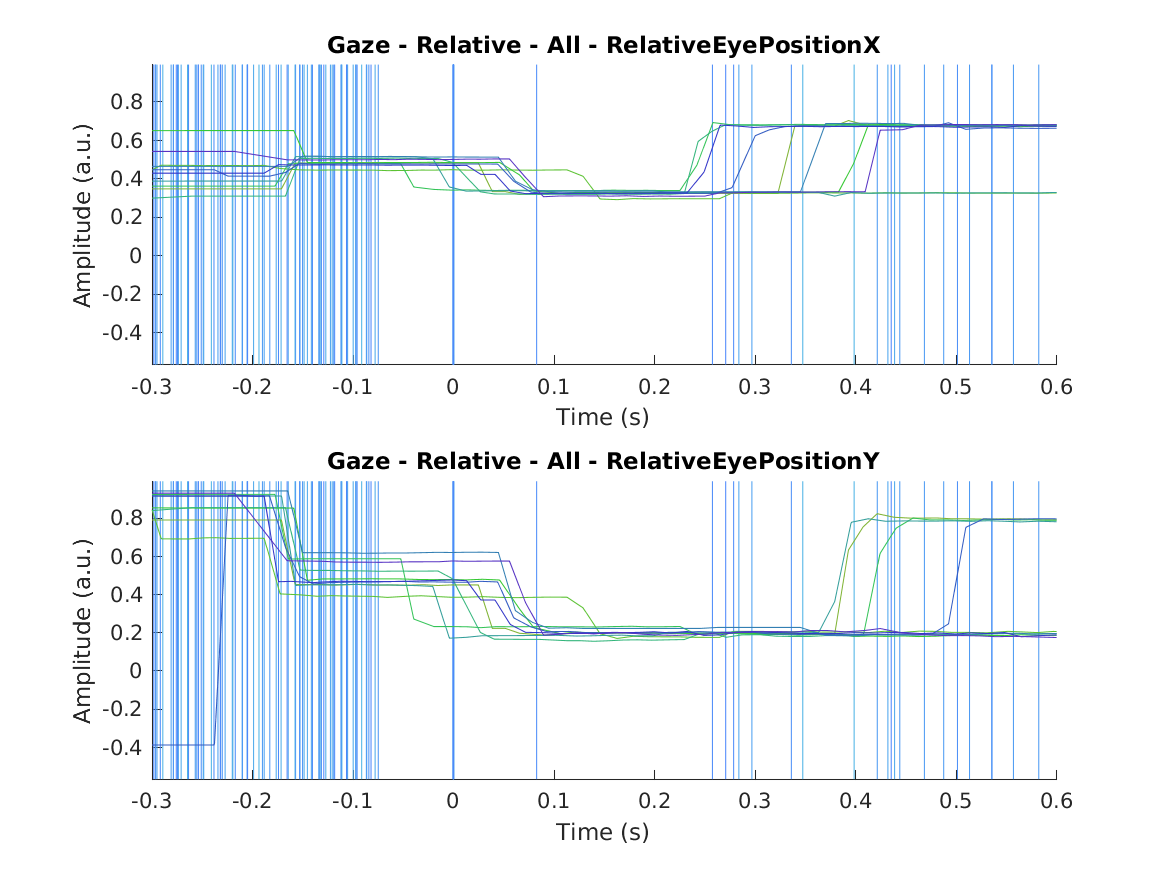
\includegraphics[width=3in]{plots/gaze-rel-all-zoom} &
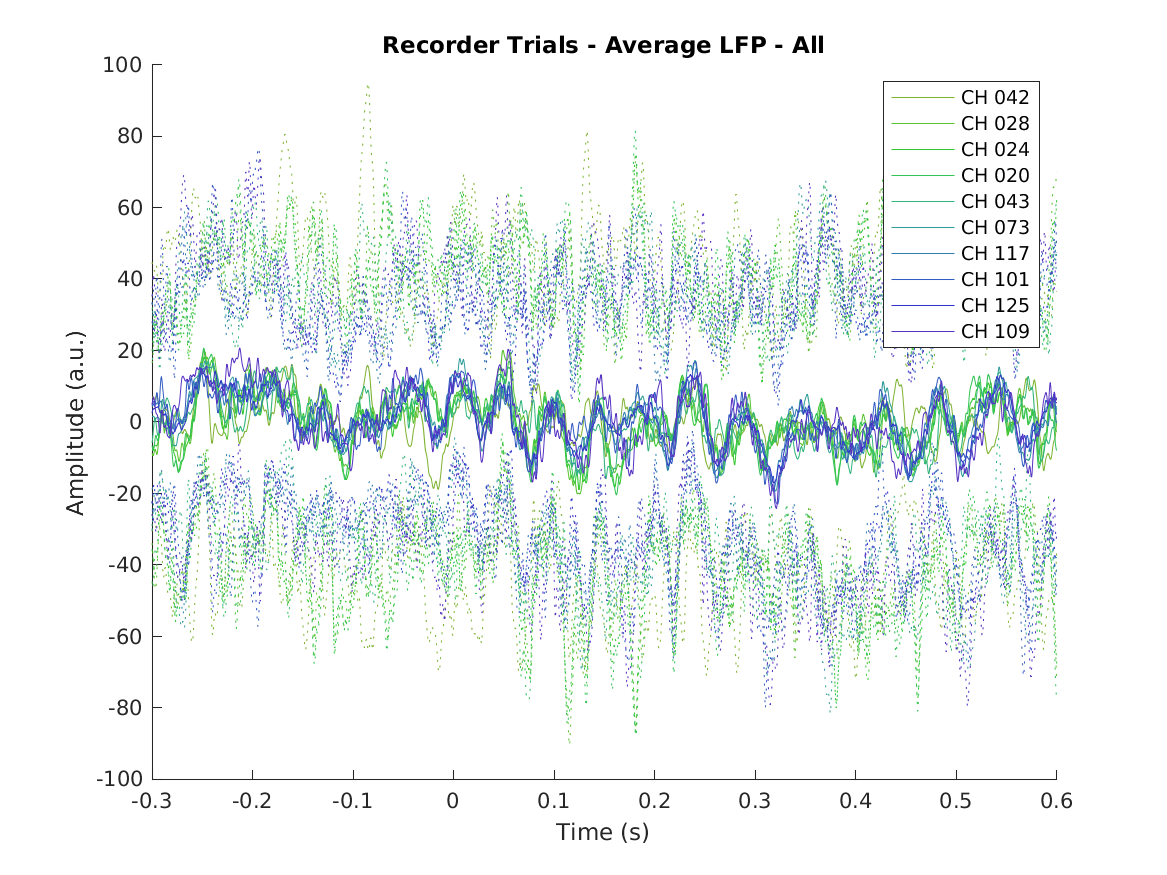
\includegraphics[width=3in]{plots/rec-avg-lfp-all-zoom} \\
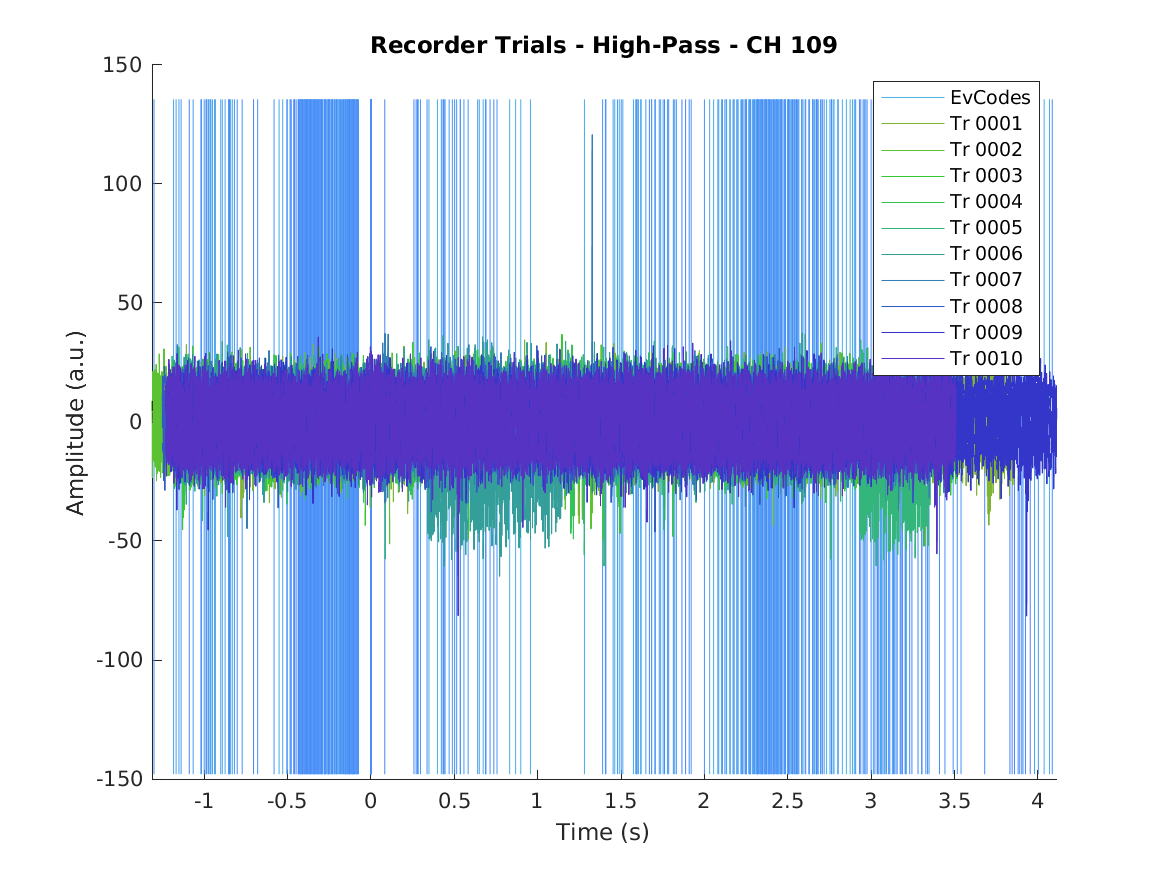
\includegraphics[width=3in]{plots/rec-hpf-CH109-full} &
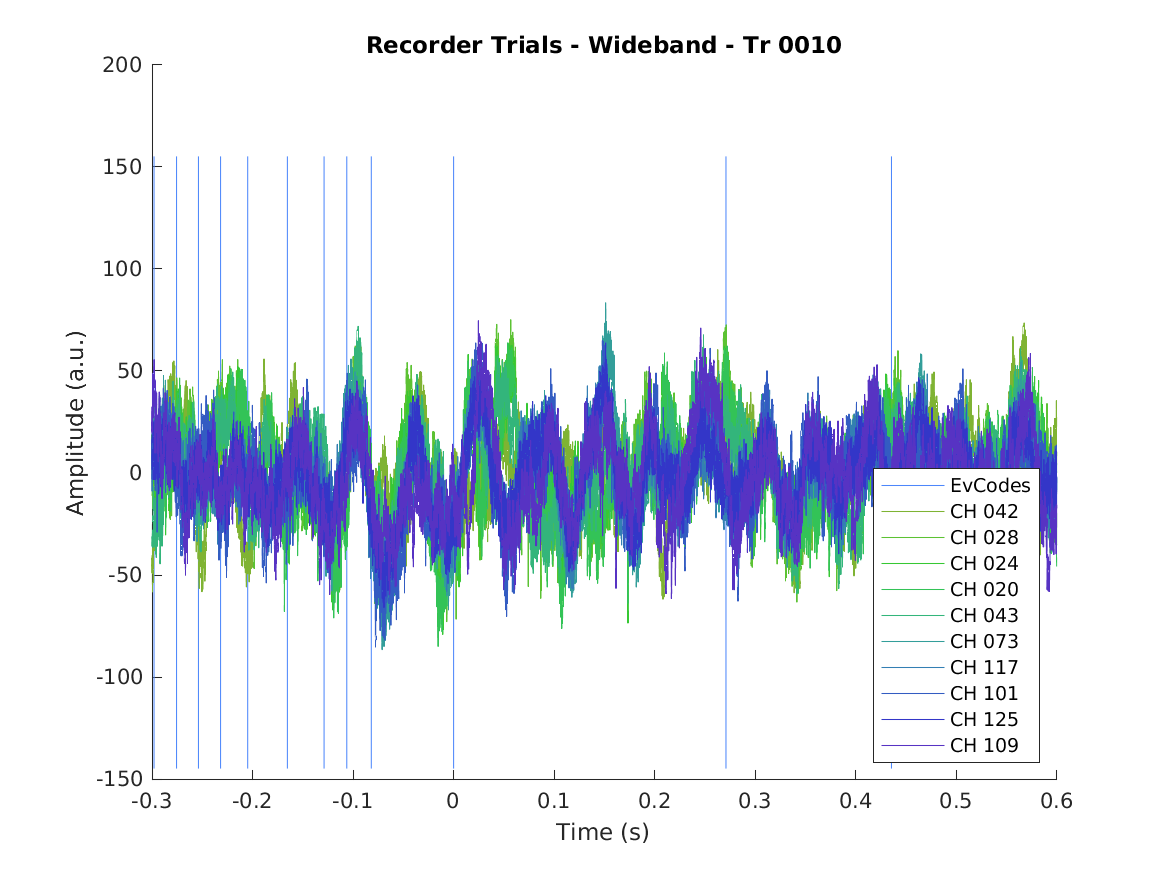
\includegraphics[width=3in]{plots/rec-wb-tr0010-zoom} \\
\end{tabular}
%
\end{center}
%
\vfill
{\tiny \input{../LICENSE.md}}
%
\clearpage
%
%
% Front matter.
%
% NOTE - Putting the overview before the TOC!
%
\pagestyle{plain}
\pagenumbering{roman}
\setcounter{page}{1}
%
% Chris's expriment utility libraries - Library reference - Overview
% Written by Christopher Thomas.

% Dummy out chapter; this is now front-matter.
\iffalse
%
\chapter{Overview}
%
\else
%
\vspace*{0.75in}
{\Huge \bfseries Overview}
\vspace*{\baselineskip}
\label{sect-over}
%
\fi

This is a set of libraries and utilities written to support ephys experiment
analyses in Thilo's lab.

This is intended to be a private project for lab-specific code that is not
specific to individual experiments. Code that lends itself to reuse outside
our lab can be migrated to public projects. Code that's experiment-specific
should be in projects associated with those experiments.

Libraries are provided in the ``\texttt{libraries}'' directory. With that
directory on path, call the \linebreak ``\texttt{addPathsExpUtilsCjt}''
function to add sub-folders.

The following sets of library functions are provided:
\begin{itemize}
%
\item \textbf{``\texttt{euAlign}''} functions (Chapter \ref{sect-align})
perform time-alignment of event lists from different sources.
%
\item \textbf{``\texttt{euChris}''} functions (Chapter \ref{sect-chris})
manipulate datasets from Chris's experiments.
%
\item \textbf{``\texttt{euFT}''} functions (Chapter \ref{sect-ft})
provide wrappers for Field Trip functions and combine commonly-used sets
of Field Trip function calls.
%
\item \textbf{``\texttt{euHLev}''} functions (Chapter \ref{sect-highlevel})
perform high-level I/O and signal processing operations. These are intended
to called instead of writing commonly-duplicated low-level processing code.
%
\item \textbf{``\texttt{euPlot}''} functions (Chapter \ref{sect-plot})
plot experiment data for testing. These don't make paper-quality plots.
%
\item \textbf{``\texttt{euTools}''} functions (Chapter \ref{sect-tools})
are helper functions used by specific tools and scripts.
%
\item \textbf{``\texttt{euUSE}''} functions (Chapter \ref{sect-use})
are functions for reading and interpreting USE data (event codes, SynchBox
activity, gaze data, and frame data).
%
\item \textbf{``\texttt{euUtil}''} functions (Chapter \ref{sect-util})
are utility functions that don't fit into other categories.
%
\end{itemize}

The following sample code is provided:
\begin{itemize}
%
\item \textbf{``\texttt{do\_read\_synchbox.m}''} -- Demonstration code for
reading SynchBox traffic saved by USE. This is described in Chapter
\ref{sect-sample-synchbox}.
%
\item \textbf{``\texttt{ft\_demo.m}''} -- Simplest practical script for
reading our lab's datasets into Field Trip. This is described in Chapter
\ref{sect-sample-demo}.
%
\end{itemize}

%
% This is the end of the file.

\clearpage
%
\tableofcontents
\clearpage
%
%
% Document parts.
%
\pagestyle{plain}
\setcounter{page}{1}
\pagenumbering{arabic}
%
\part{Examples}
\label{sect-samples}
%
\input{eucjt-libs-sample-demo}
%
\part{Library Functions}
\label{sect-libs}
%
\input{eucjt-libs-align}
\input{eucjt-libs-ft}
\input{eucjt-libs-plot}
\input{eucjt-libs-tools}
\input{eucjt-libs-use-notes}
\input{eucjt-libs-use}
\input{eucjt-libs-util}
%
%
\end{document}

%
% This is the end of the file.
